\ifx\flag\undefined
	\documentclass{easyclass}
	\begin{document}
\else
	\chapter{Quantum Algorithms}
\fi

The general quantum computing process is shown in Figure \ref{fig:quantum computing}. If we consider the preparation of qubit as an initial step, the \textbf{basic framework of quantum algorithm} can be summarized as follows:
\begin{enumerate}[(1)]
	\item The system will \textcolor{red}{start with} the qubits in a particular \textcolor{red}{classical state};
	\item From there the system is put into a \textcolor{red}{superposition of many states};
	\item This is followed by acting on this superposition with several \textcolor{red}{unitary operations};
	\item And finally, a \textcolor{red}{measurement} of the qubits.	
\end{enumerate}

\begin{figure}[h]
	\centering
	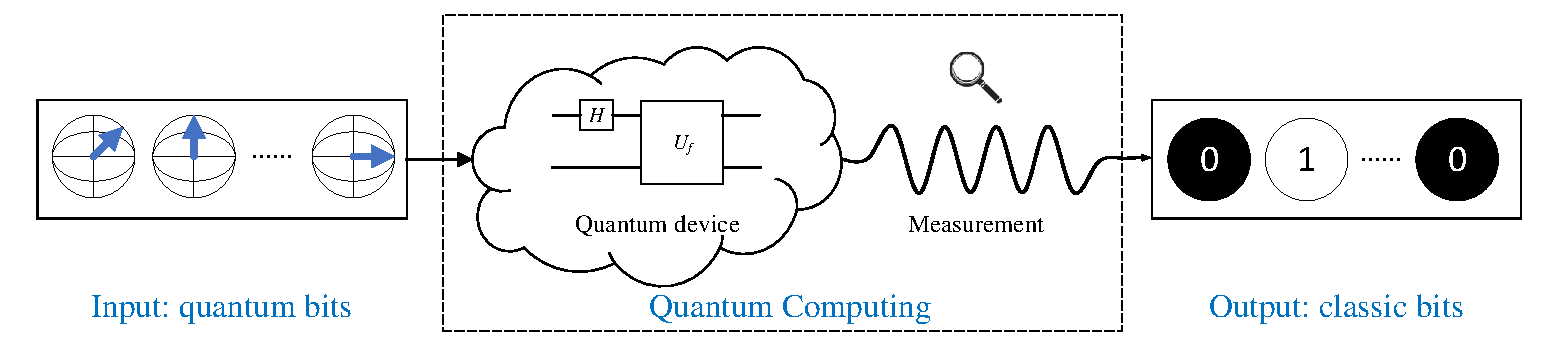
\includegraphics[width=\textwidth]{quantum-computing}
	\caption{Quantum computing}
	\label{fig:quantum computing}
\end{figure}	
	
\section{Deutsch's Algorithm}
\subsection{The Deutsch oracle problem}
The simplest quantum algorithm is Deutsch’s algorithm, which is a nice algorithm that solves a slightly contrived problem. This algorithm is concerned with functions from the set $\{0,1\}$ to the set $\{0,1\}$. There are four different implementations that belong to a function $f:\{0,1\}\rightarrow \{0,1\}$.

\begin{figure}[h]
	\centering
	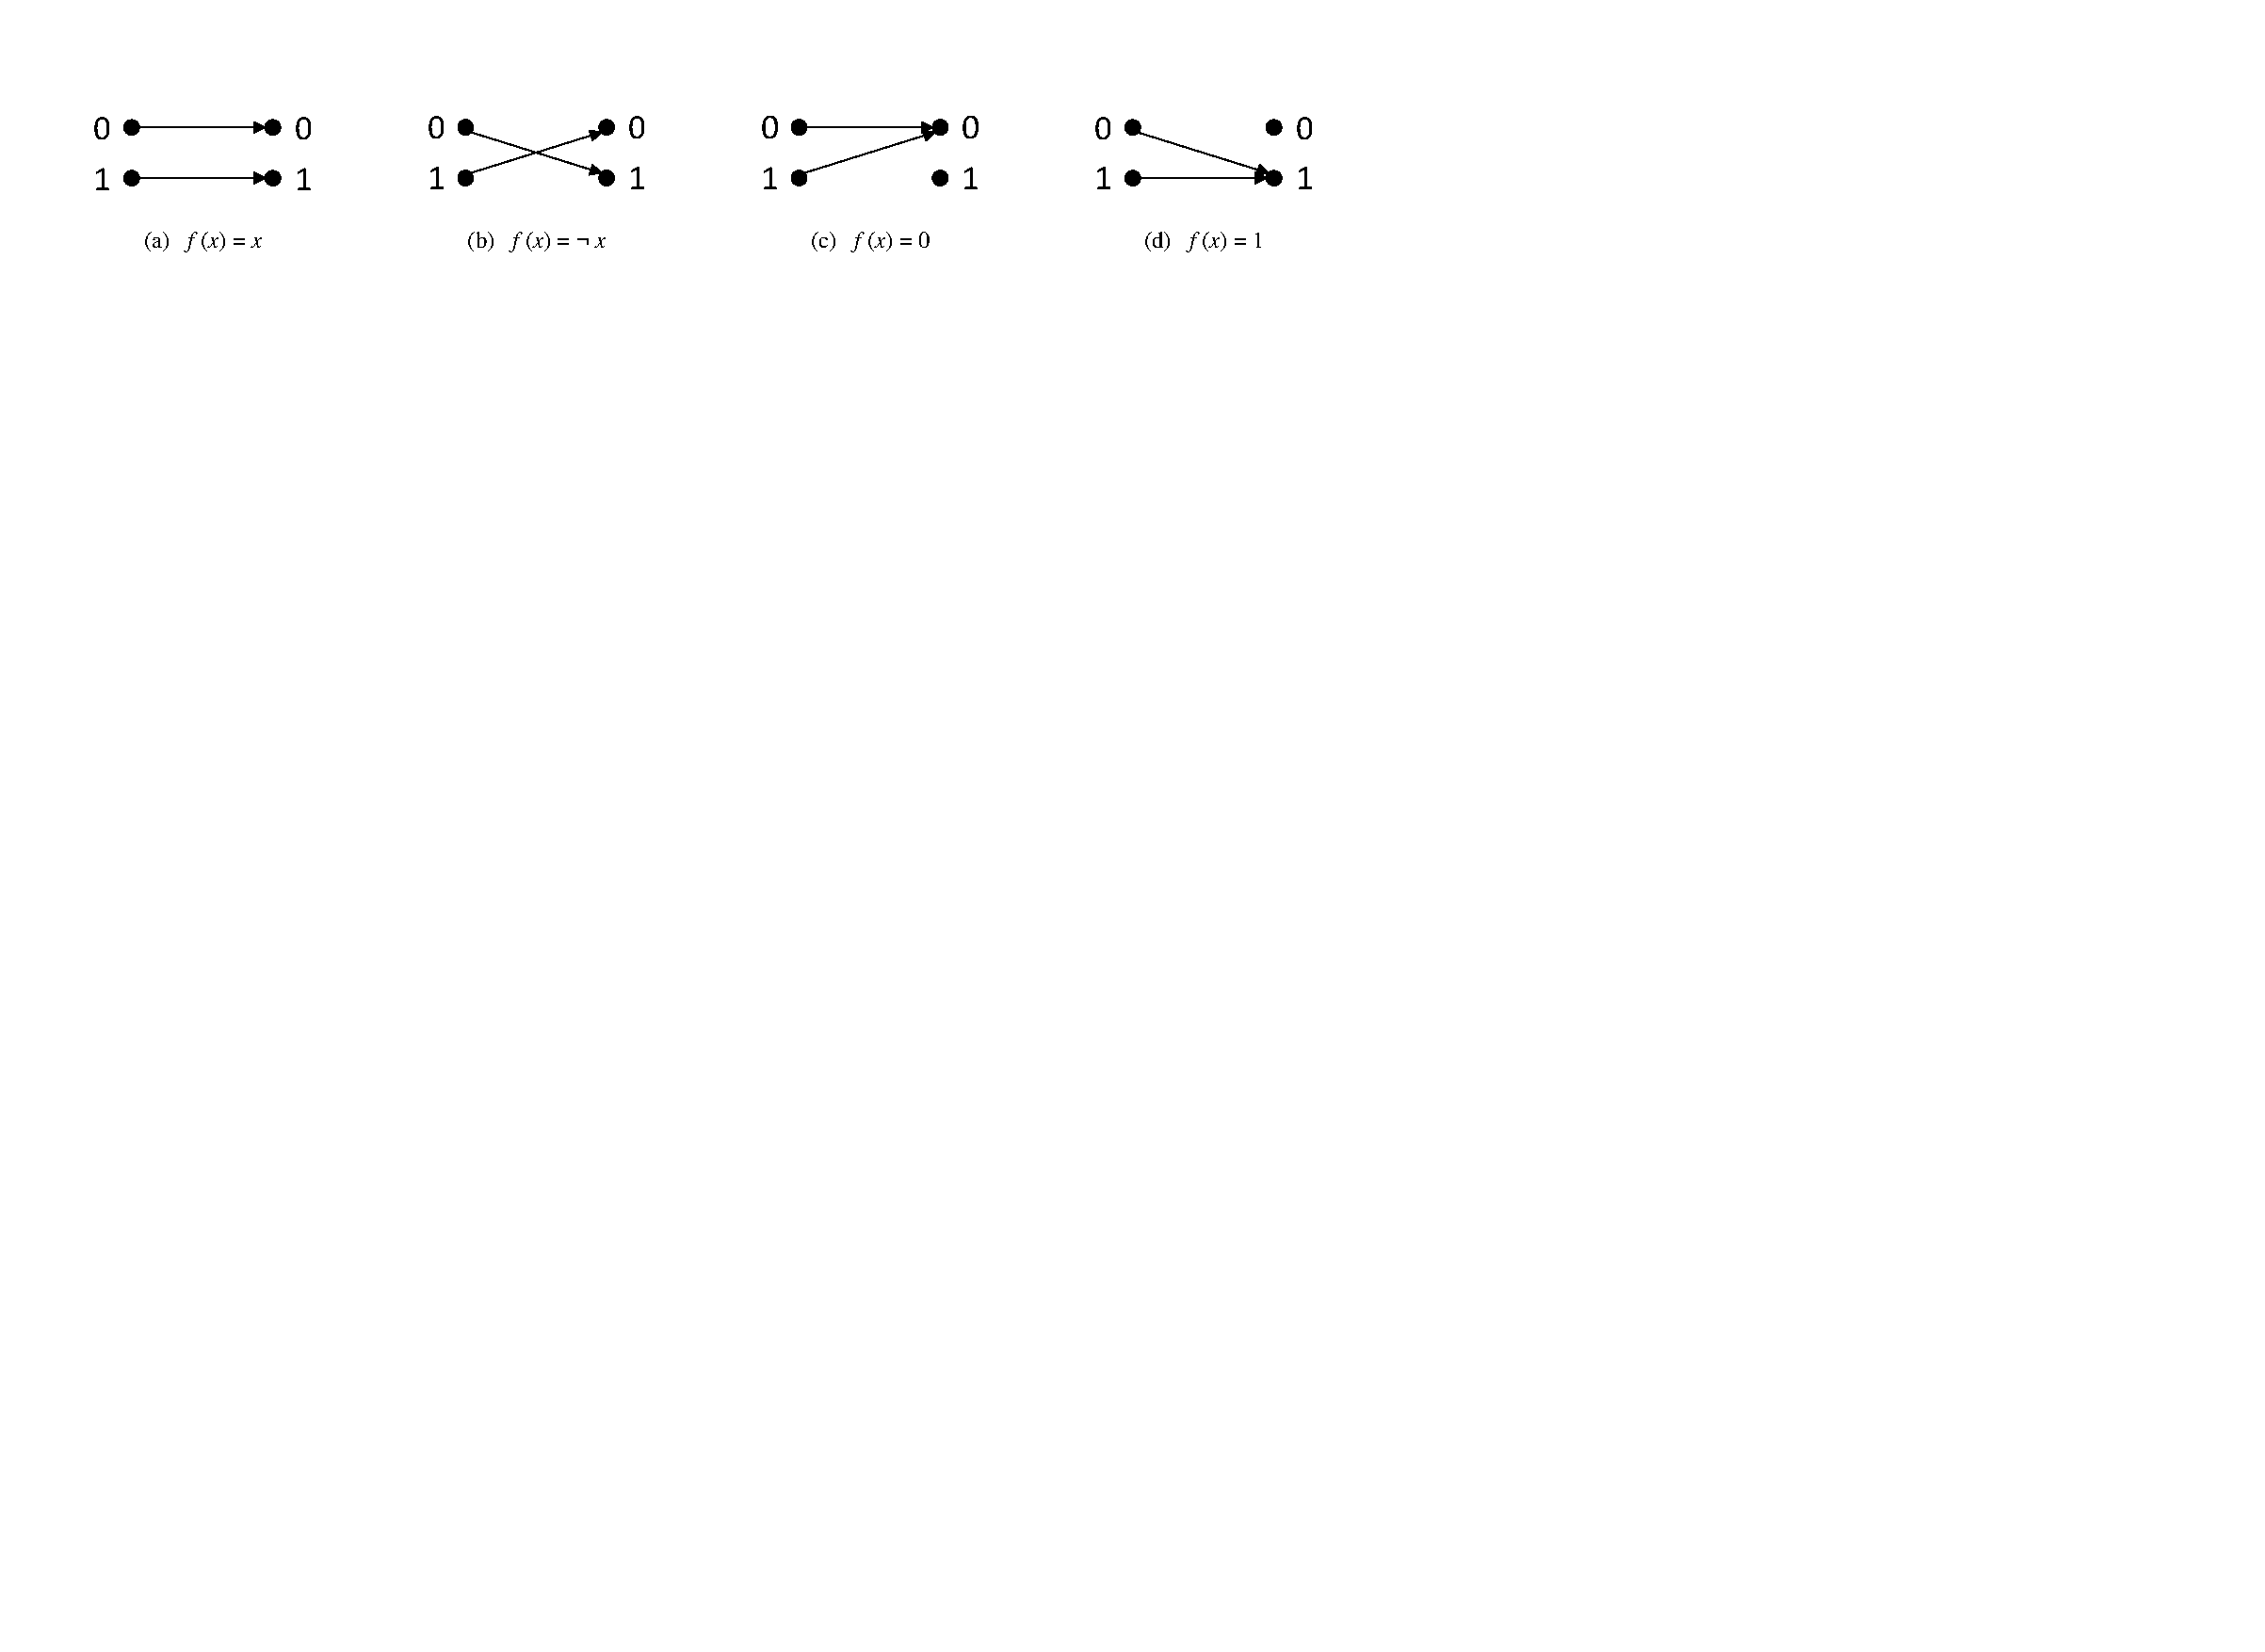
\includegraphics[width=\textwidth]{balanced-constant}
	\caption{Balanced and constant functions}
	\label{fig:balanced constant}
\end{figure}

\textbf{Balanced and constant functions}: as shown in Figure \ref{fig:balanced constant}, the first two functions, \textit{i.e.}, identity function $f(x)=x$ and negation function $f(x)=\neg x$, are called \textbf{balanced} since $f(0)\neq f(1)$. In contrast, the last two functions, \textit{i.e.}, constant-0 function $f(x)=0$ and constant-1 function $f(x)=1$, are called \textbf{constant} since $f(0)=f(1)$.

\textbf{The Deutsch oracle problem}: given a function $f:\{0,1\}\rightarrow \{0,1\}$ as a black box (BB), where one can evaluate an input, but cannot ``look inside'' and ``see'' how the function is defined, determine if the function is \textbf{balanced} or \textbf{constant}. 

\textbf{Solution with a classic computer}: as shown in Figure \ref{fig:solution with a classic computer}, first, evaluate $f(x)$ on one input; second, evaluate $f(x)$ on the second input, compare the outputs and make the decision. This means a classic computer needs \textbf{two-step operations} to solve the Deutsch oracle problem. How about a quantum computer?

\begin{figure}[h]
	\centering
	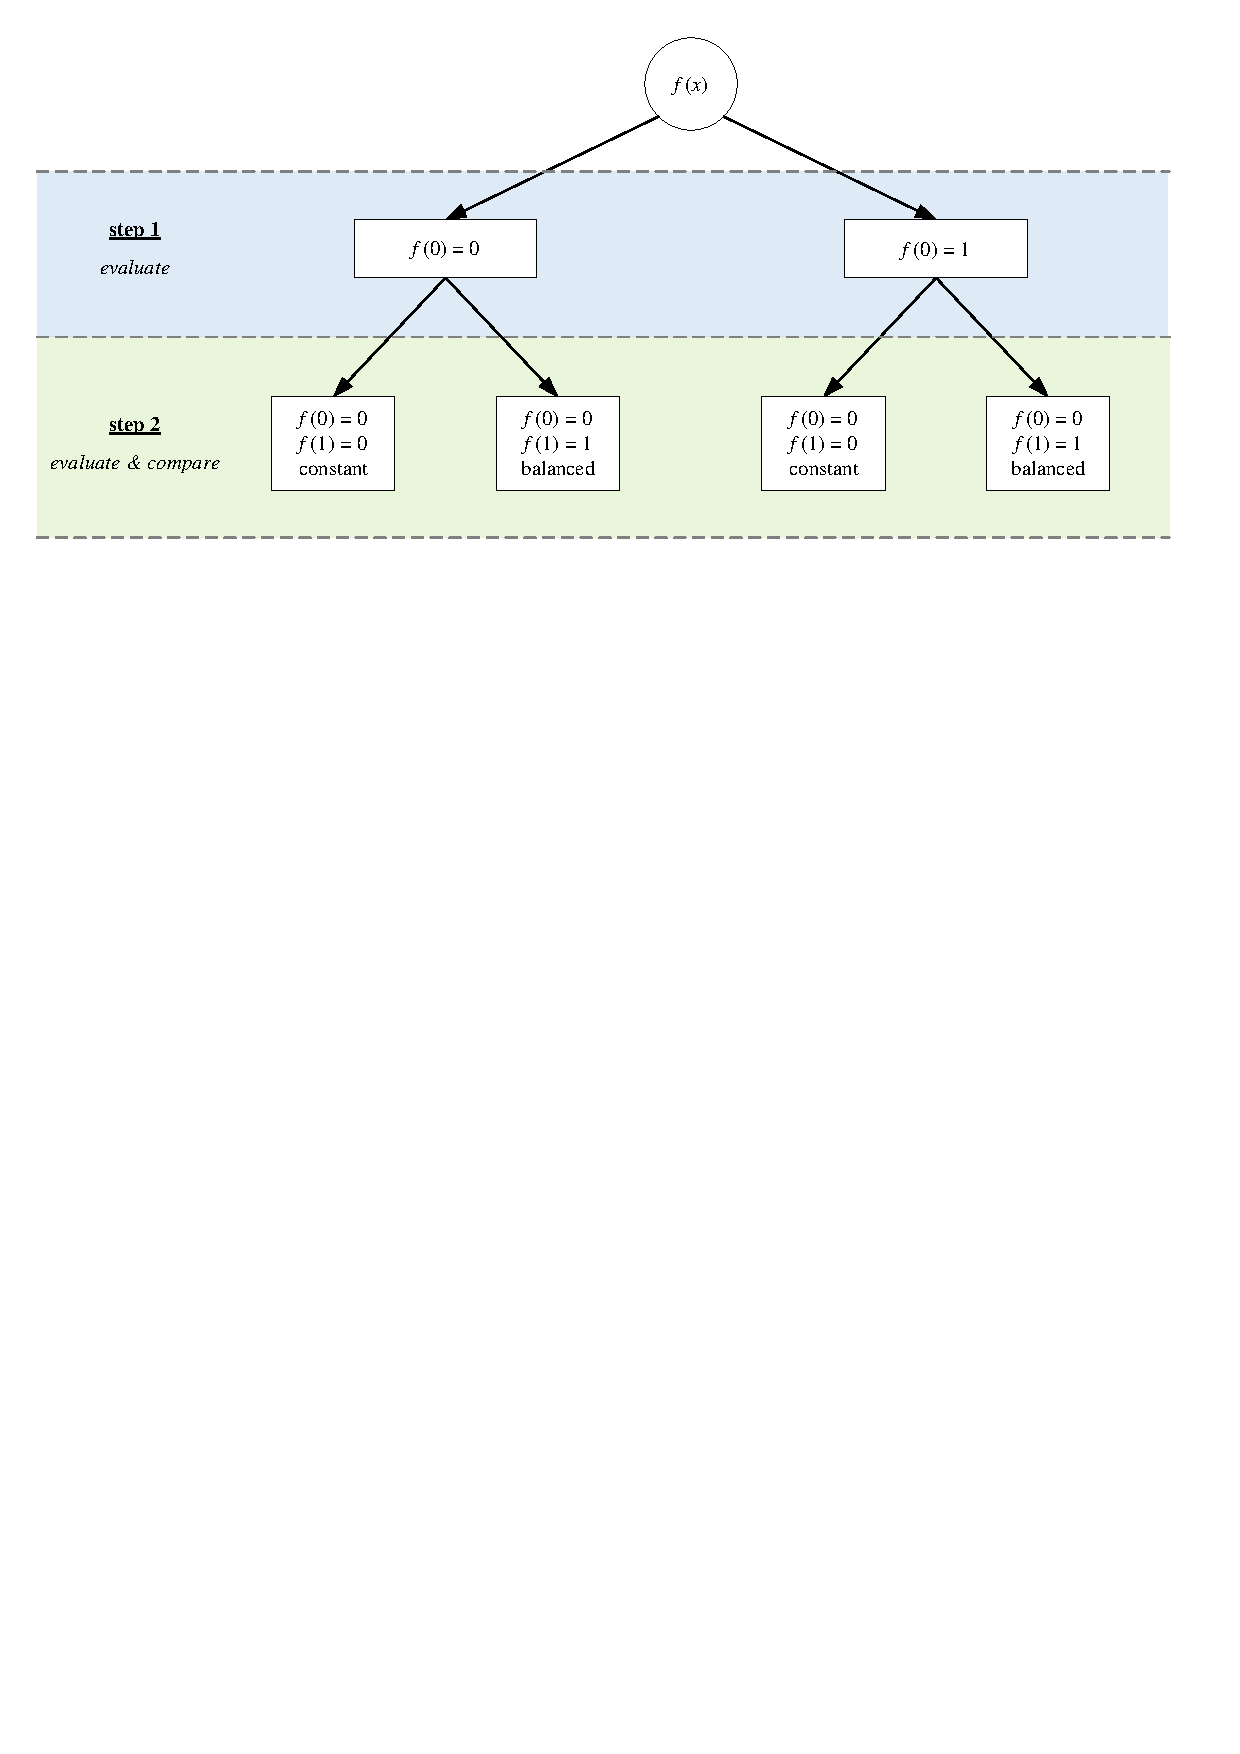
\includegraphics[width=\textwidth]{solution-classic}
	\caption{Solution with a classic computer}
	\label{fig:solution with a classic computer}
\end{figure}

\subsection{Reversible and irreversible operators}
%Quantum computer use only reversible operations, which means given the operation and output value, we can find the input value. 

\textbf{reversible operations}: Operations which permute are reversible, \textit{e.g.}, NOT gate, CNOT gate, Hardmard gate, identity and negation gates.

\begin{example}[NOT (X) gate]{eg:X gate}
	\textbf{X gate} is a logic gate which implements logical negation. It outputs a bit opposite of the bit that is put into it. 
	\begin{equation}
			\mathbf{X}\ket{0}=
			\begin{bmatrix}
				0 & 1\\
				1 & 0
			\end{bmatrix} 
			\begin{bmatrix}
				1 \\ 0
			\end{bmatrix}=
			\begin{bmatrix}
				0 \\ 1
			\end{bmatrix}=\ket{1}
			\quad\Longleftrightarrow\quad
			\mathbf{X}\ket{1}=
			\begin{bmatrix}
				0 & 1\\
				1 & 0
			\end{bmatrix} 
			\begin{bmatrix}
				0 \\ 1
			\end{bmatrix}=
			\begin{bmatrix}
				1 \\ 0
			\end{bmatrix}=\ket{0}
	\end{equation}
\end{example}

\begin{example}[Hardmard (H) gate]{ex:H gate}
	\textbf{H gate} maps a $0$- or $1$-bit into exactly equal superposition, and back (operations are their own inverse!)
	\begin{equation}
		\begin{cases}
			\mathbf{H}\ket{0}=
			\begin{bmatrix}
				\frac{1}{\sqrt{2}} & \frac{1}{\sqrt{2}}\\
				\frac{1}{\sqrt{2}} & -\frac{1}{\sqrt{2}}
			\end{bmatrix} 
			\begin{bmatrix}
				1 \\ 0
			\end{bmatrix}=
			\begin{bmatrix}
				\frac{1}{\sqrt{2}} \\ \frac{1}{\sqrt{2}}
			\end{bmatrix}
			\ \,\,\Longleftrightarrow
			\ \,\,\mathbf{H}\begin{bmatrix}
				\frac{1}{\sqrt{2}} \\ \frac{1}{\sqrt{2}}
			\end{bmatrix}=
			\begin{bmatrix}
				\frac{1}{\sqrt{2}} & \frac{1}{\sqrt{2}}\\
				\frac{1}{\sqrt{2}} & -\frac{1}{\sqrt{2}}
			\end{bmatrix} 
			\begin{bmatrix}
				\frac{1}{\sqrt{2}} \\ \frac{1}{\sqrt{2}}
			\end{bmatrix}=
			\begin{bmatrix}
				1 \\ 0
			\end{bmatrix}=\ket{0}
			\\\\
			
			\mathbf{H}\ket{1}=
			\begin{bmatrix}
				\frac{1}{\sqrt{2}} & \frac{1}{\sqrt{2}}\\
				\frac{1}{\sqrt{2}} & -\frac{1}{\sqrt{2}}
			\end{bmatrix} 
			\begin{bmatrix}
				0 \\ 1
			\end{bmatrix}=
			\begin{bmatrix}
				\frac{1}{\sqrt{2}} \\ -\frac{1}{\sqrt{2}}
			\end{bmatrix}
			\Longleftrightarrow
			\mathbf{H}\begin{bmatrix}
				\frac{1}{\sqrt{2}} \\ -\frac{1}{\sqrt{2}}
			\end{bmatrix}=
			\begin{bmatrix}
				\frac{1}{\sqrt{2}} & \frac{1}{\sqrt{2}}\\
				\frac{1}{\sqrt{2}} & -\frac{1}{\sqrt{2}}
			\end{bmatrix} 
			\begin{bmatrix}
				\frac{1}{\sqrt{2}} \\ -\frac{1}{\sqrt{2}}
			\end{bmatrix}=
			\begin{bmatrix}
				0 \\ 1
			\end{bmatrix}=\ket{1}
		\\
		\end{cases}
	\end{equation}
	From the above equations, we have three findings:
	\begin{itemize}
		\item We can transition into superposition from classic state, \textit{i.e.}, $\ket{0}$ or $\ket{1}$;
		\item We can transition out of superposition without measurement;
		\item We can structure quantum computation results deterministically instead of probabilistically.
	\end{itemize}
\end{example}


\textbf{The unit circle state machine} is a unit circle with $8$ states, of which only $4$ states are mutually different as shown in Figure \ref{fig:unit circle state machine}(a). Its state transitions under X gate is shown in Figure \ref{fig:unit circle state machine}(b), and the state transitions under H gate is shown in Figure \ref{fig:unit circle state machine}(c).
\begin{figure}[h]
	\centering
	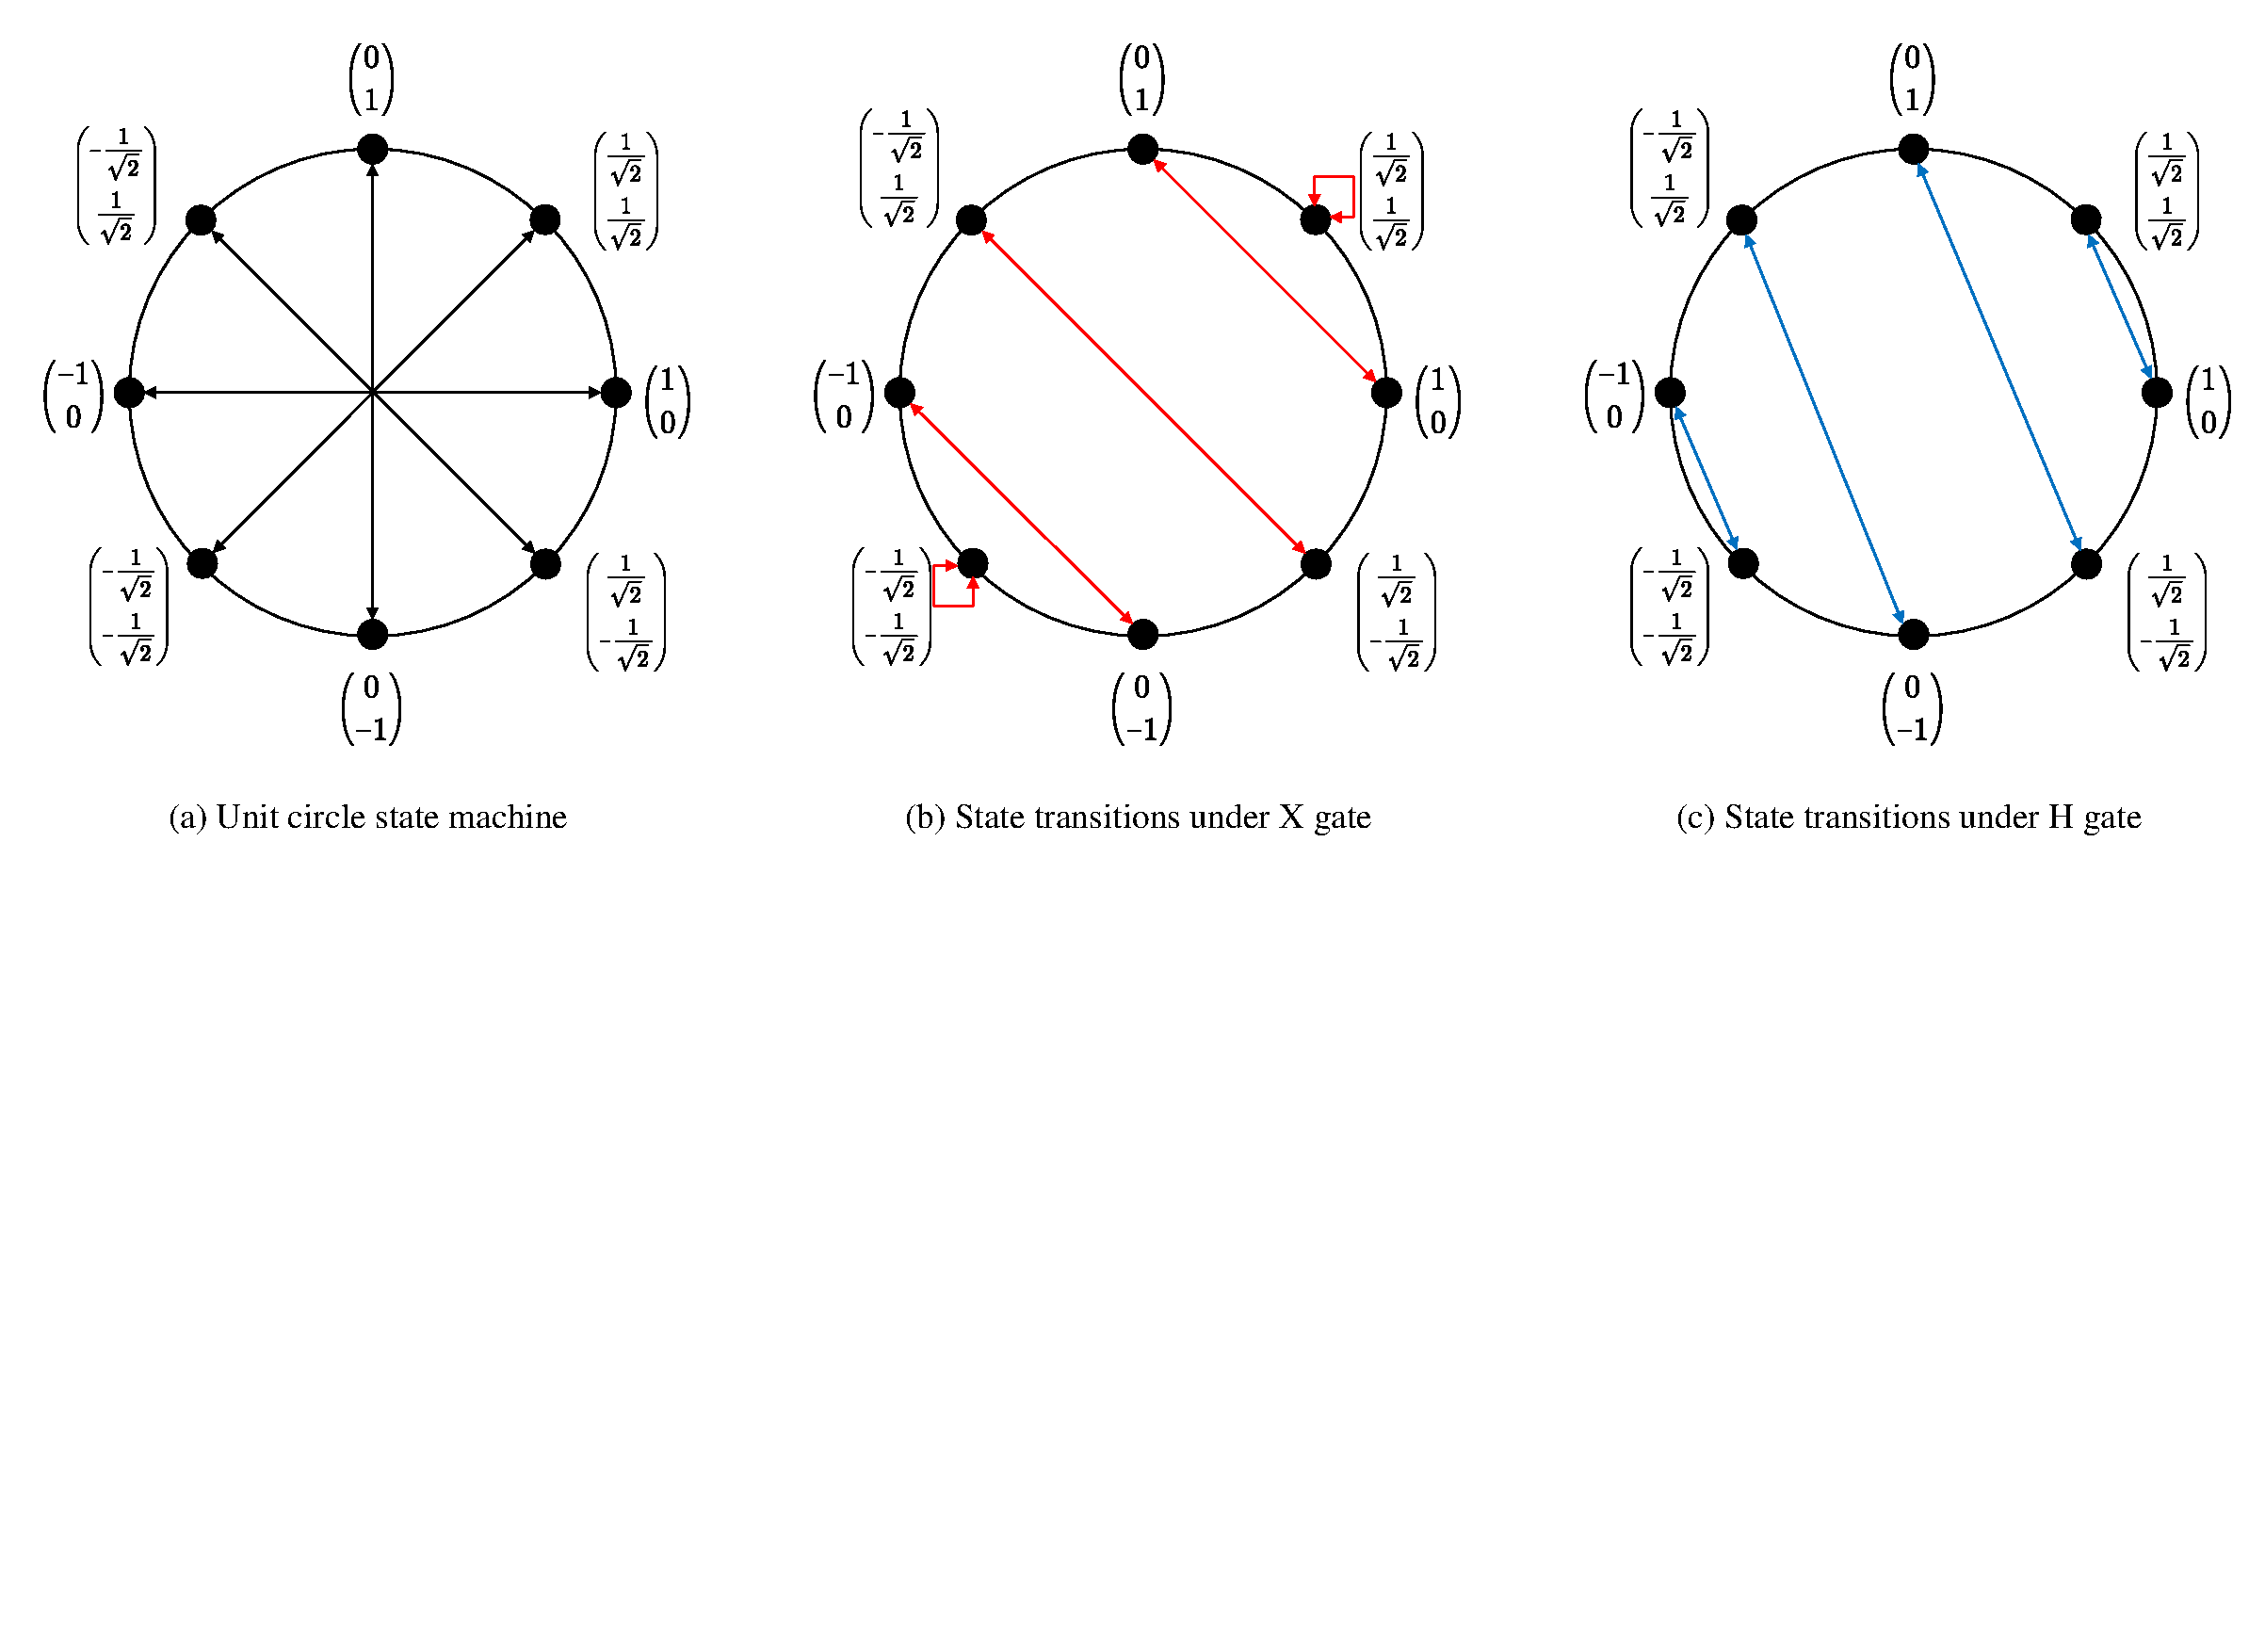
\includegraphics[width=\textwidth]{unit-circle-state-machine}
	\caption{The unit circle state machine}
	\label{fig:unit circle state machine}
\end{figure}

Given a quantum circuit consisting of only X and H gates, its state transition trajectory can be conveniently inferred using the rules described by Figure \ref{fig:quantum circuit example} 
\begin{figure}[h]
	\centering
	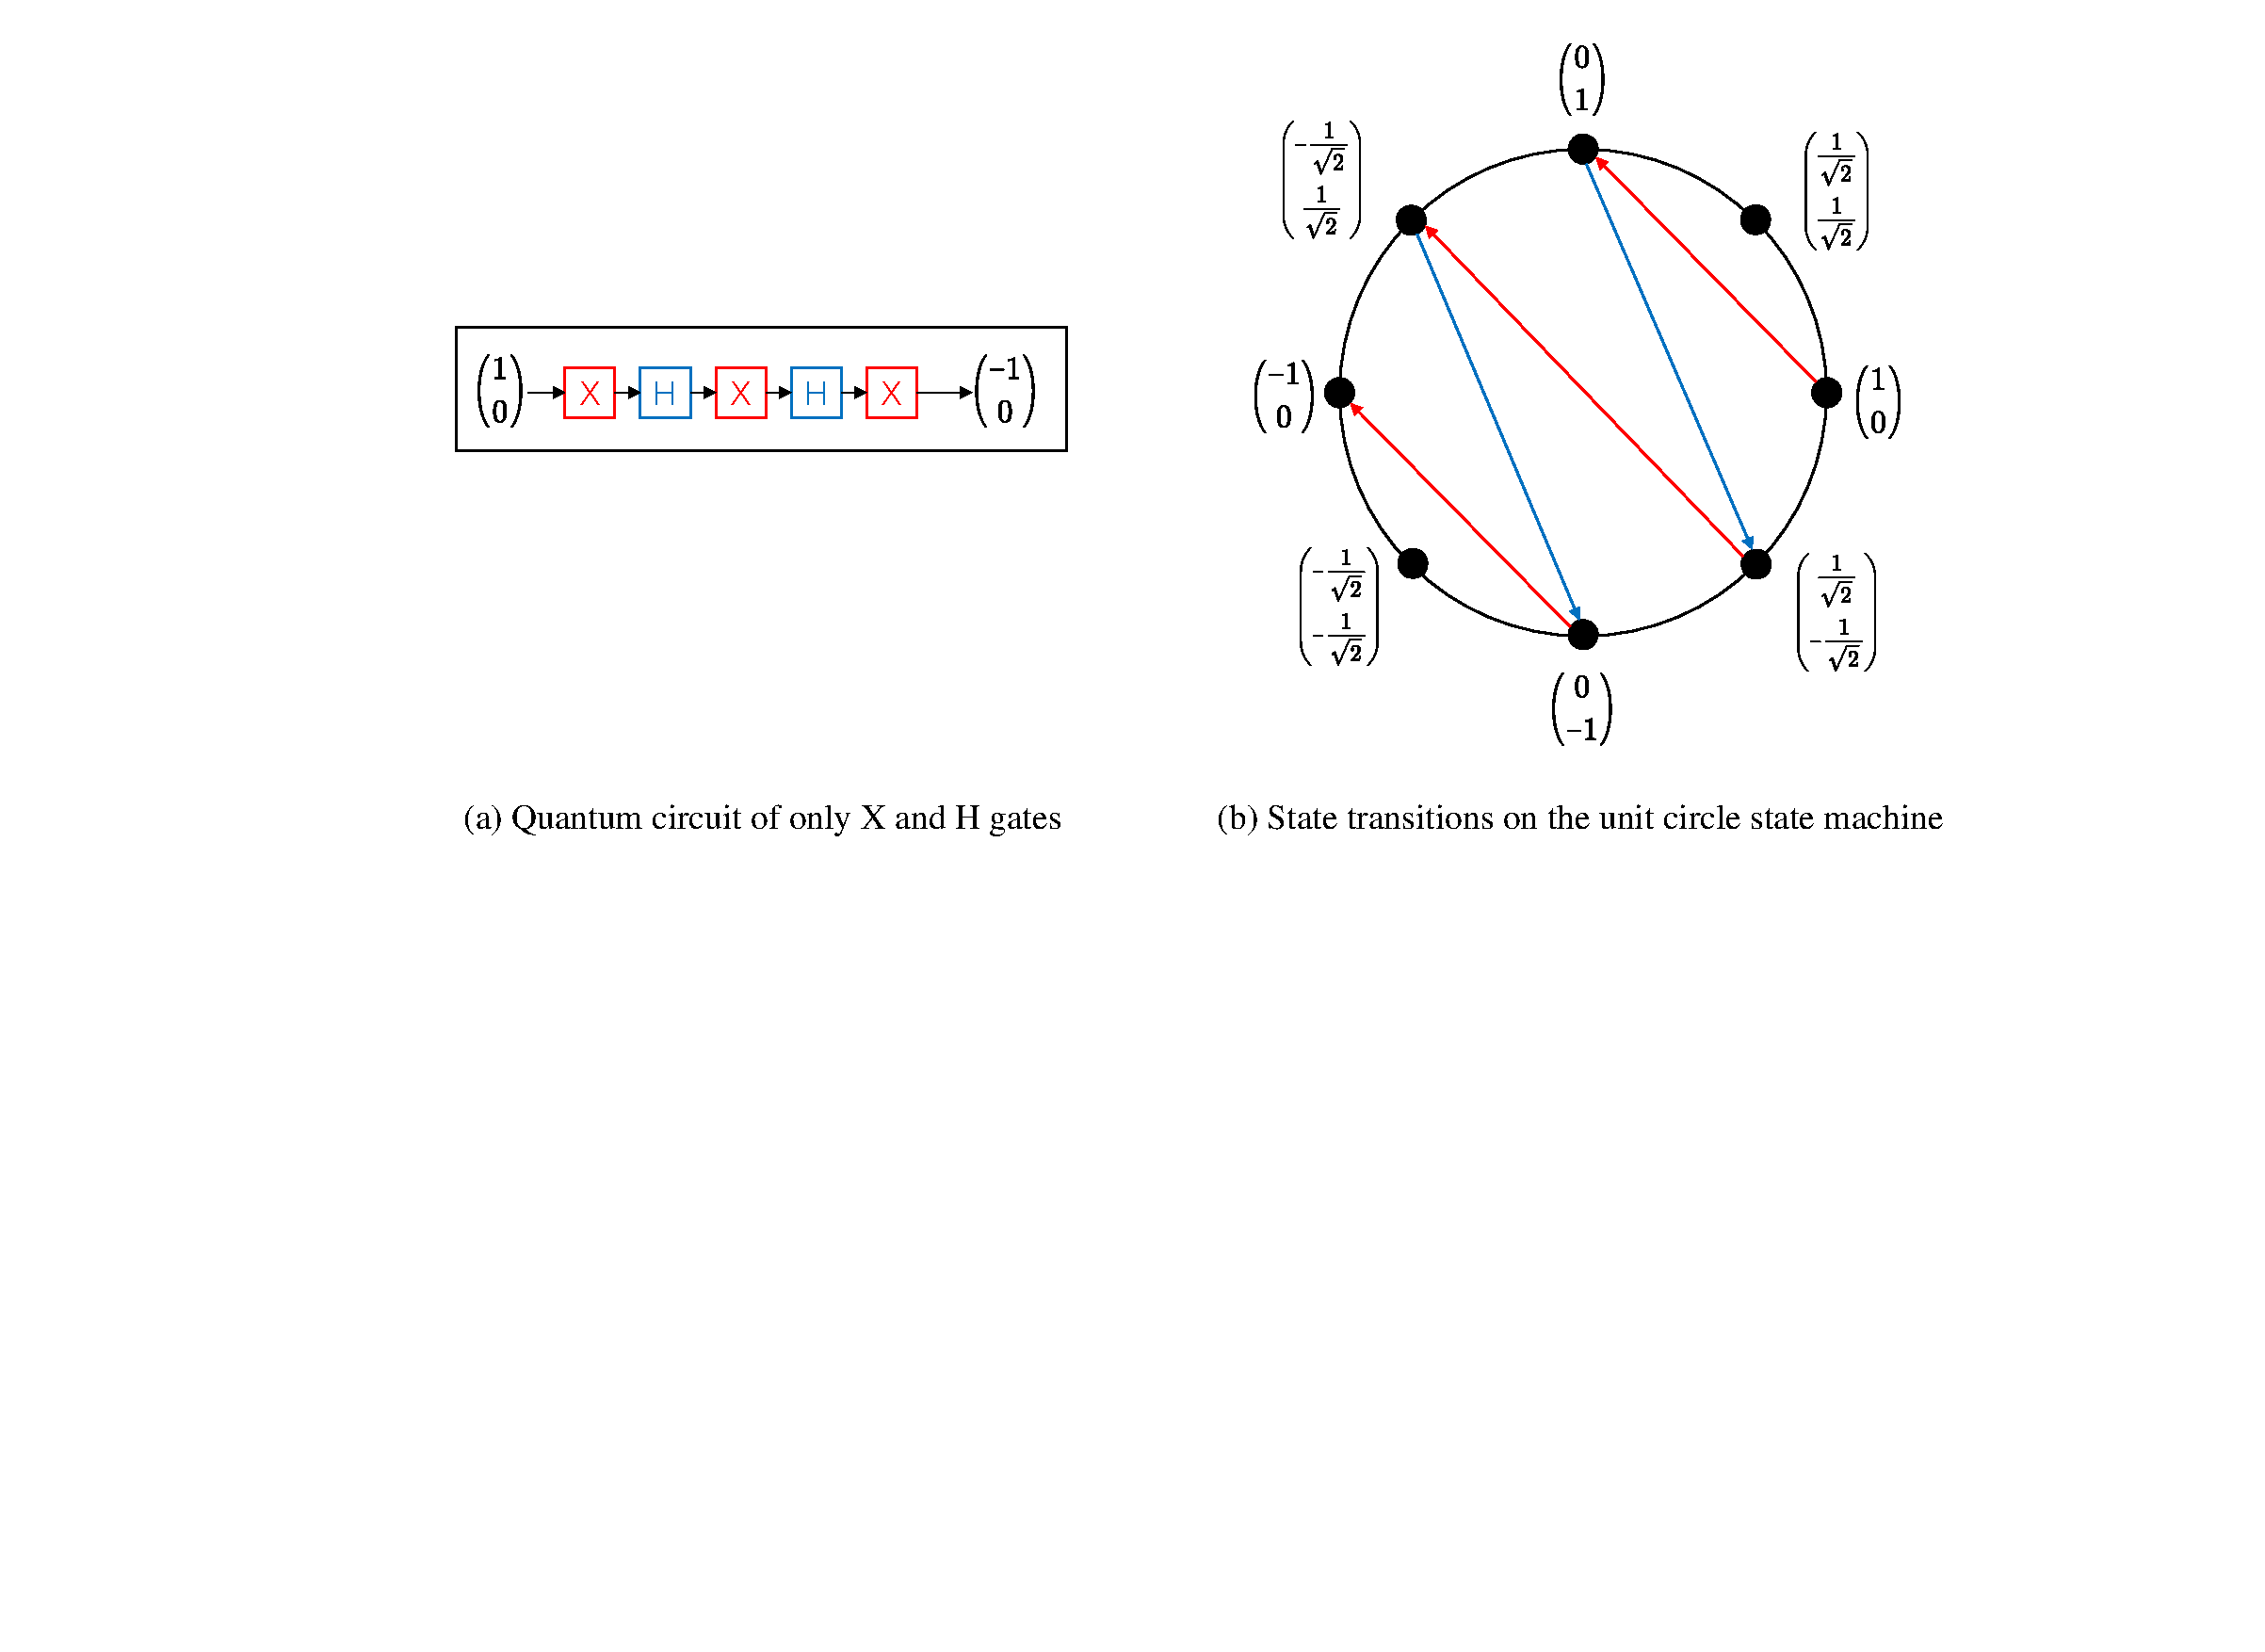
\includegraphics[width=\textwidth]{quantum-circuit-example}
	\caption{The fast calculation with the help of unit circle state machine}
	\label{fig:quantum circuit example}
\end{figure}


\textbf{irreversible operations}: Operations which erase \& overwrite are irreversible, \textit{e.g.}, constant-0 and constant-1 gates.




\subsection{Deutsch's algorithm}
\subsection{Discussion}

\section{Deutsch-Jozsa Algorithm}	
\subsection{Hadamard matrix and Kronecker product}
\subsection{N-bit Deutsch oracle problem}
\subsection{Deutsch-Jozsa algorithm}
	
	
	
\curinstructor{Chao Liang}
	
\ifx\flag\undefined
	\end{document}
\else